%!TEX root = ../thesis.tex
%*******************************************************************************
%****************************** Second Chapter *********************************
%*******************************************************************************

\chapter{Results of Physical Properties Modification in Novel 2D materials \label{chap:5}}

\ifpdf
    \graphicspath{{Chapter5/Figs/Raster/}{Chapter5/Figs/PDF/}{Chapter5/Figs/}{Chapter5/Figs/Vector/}}
\else
    \graphicspath{{Chapter5/Figs/Vector/}{Chapter5/Figs/}}
\fi

\section{Number of layers and types of stackings}
\subsection[Few-layer of Calcium hydroxide]{Few-layer of Calcium hydroxide \footcite[This work is published in:][]{Aierken2015.porlandite}}
\subsection[Few-layer of pentasilicene]{Few-layer of pentasilicene \footcite[This work is published in:][]{Aierken2016.pentasilicene}}

\section{Mechanical strain}
\subsection[Variation of vibrational modes under strain in phosphorene]{Variation of vibrational modes under strain in phosphorene \footcite[This work is published in:][]{Aierken2015.thermalP}}

In \autoref{sec:pho_phos} we calculated the phonon dispersion of black and blue phosphorene, here we will discuss how the vibrational modes change with strain. In \autoref{fig:ire_phos} we revisit the phonon dispersion of phosphorene, here the $\Gamma$ point vibrational modes with their irreducible representations and their frequencies are given.

\begin{figure}[htbp]
\centering
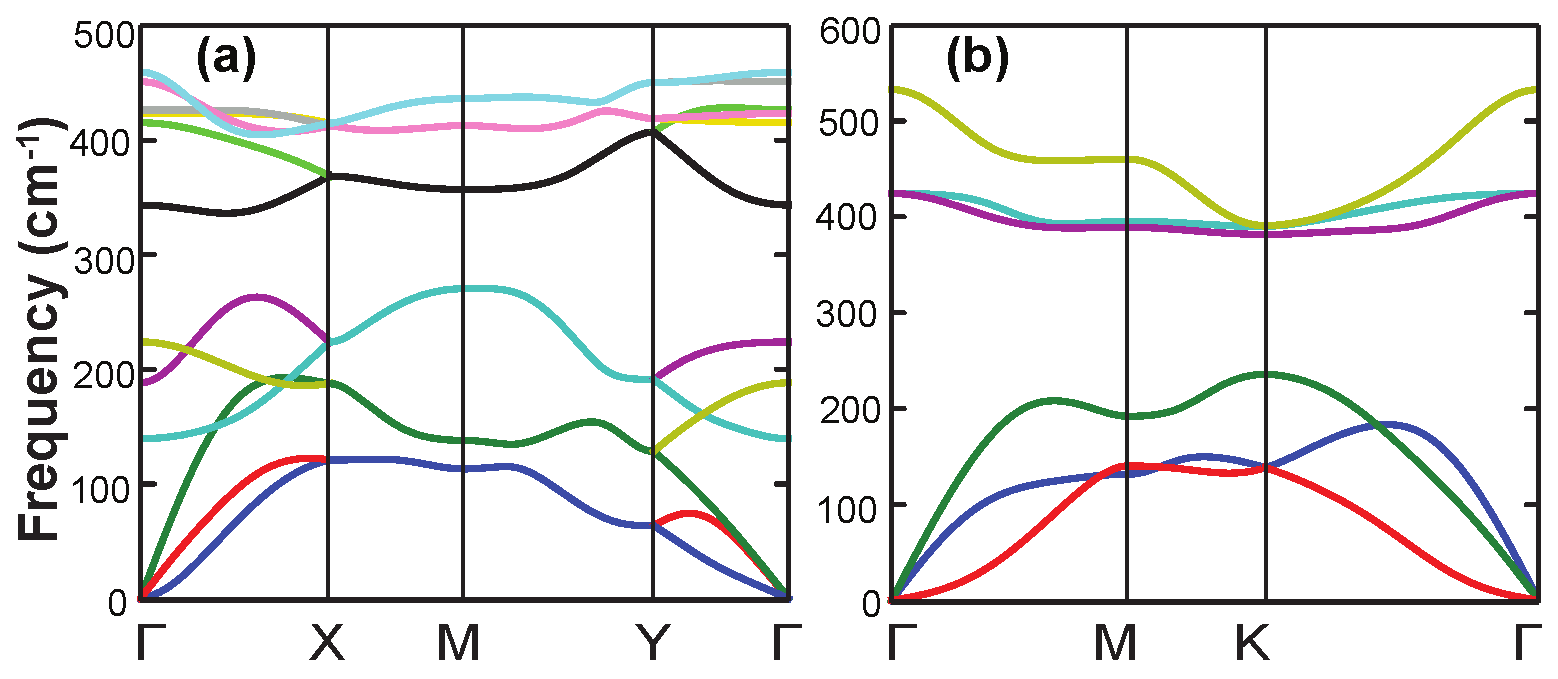
\includegraphics[width=0.8\linewidth]{phos_phon.eps}%
\caption{Calculated phonon dispersions for prinstine (a) black and (b) blue P. (c) Optical phonon modes together with their frequencies (in units of cm$^{-1}$) at the $\Gamma$ point and irreducible representations for black P and blue P. (c) Optical phonon modes together with their frequencies (in units of cm$^{-1}$) at the $\Gamma$ point and irreducible representations for black P and blue P.\label{fig:ire_phos}}
\end{figure}

\begin{figure}[htbp]
\centering
\includegraphics[width=0.8\linewidth]{strain_vib.eps}%
\caption{ (Color online) Variation of the $\Gamma$ frequencies with strain: (a) zigzag and (b) armchair direction of black P and (c) blue P.  \label{fig:shift_phos} }
\end{figure}

With the knowledge of the space group and its character table it is possible to assign vibrational modes to each band at the $\Gamma$-point. A table of all optical modes together with its frequency and irreducible representation for both structures is presented in \autoref{fig:ire_phos}(c) for the strainless structures. In \autoref{fig:shift_phos}, we show the variation of these optical phonons at the $\Gamma$ point under uniaxial strain. Our calculations agree well with the results of Ref.~\cite{phonon-blackP-1}. The frequency shift by strain can be directly detected using Raman spectroscopy. 
Depending on the atomic motion of the modes, the magnitude and type of strain, we find that the dependence of the phonon frequency can be different for each mode. Especially, the higher energy optical modes under uniaxial strain, applied along the zigzag direction, exhibit a much larger variation, see \autoref{fig:shift_phos}(a). B$^2_{3g}$ mode of black P has a different behavior under tensile and compressive strains along the zigzag direction. Applying a tensile (compressive) strain increases (decreases) the frequency of B$^2_{3g}$ mode. The frequency spacing between A$^2_{g}$ and B$_{2u}$ modes decreases when black P is stretched along both zigzag and armchair directions. While  the frequency of A$^2_{g}$ mode exhibits almost no variation under strain applied along the armchair direction,  it significantly varies under  strain applied along the zigzag direction.
Among the low lying optical modes (i.e., B$_{1u}$, B$_{1g}$ and B$^1_{3g}$), the B$_{1u}$ mode exhibits a larger variation with applied strain. 
E$_g$ and A$_{1g}$ modes of blue P always are red shifted when changing strain from compressive to tensile. Our results show that by measuring the frequency shift in the particular modes, it is possible to determine the
strain distribution in phosphorene.  

Our results show that the frequency shift observed in particular modes can be utilized to determine strain distribution in phosphorene.

\subsection[Carrier mobility enhancement in TiS$_3$ monolayer with strain]{Carrier mobility enhancement in TiS$_3$ monolayer with strain \footcite[This work is published in:][]{Aierken2016.mobility}}
\subsection[Magnetic properties modulation in penta-hexa-graphnene with strain]{Magnetic properties modulation in penta-hexa-graphnene with strain \footcite[This work is published in:][]{Aierken2016.magnetism}}

\section{Adatom adsorption}
\subsection[Nitrogen edge-decorated graphene nanoribbon]{Nitrogen edge-decorated graphene nanoribbon \footcite[This work will be published as:][]{Aierken2017.GNR}}

\section{Heterostructures}
\subsection[Electrical transport in 1T/2H/1T MoS2 lateral heterostructure]{Electrical transport in 1T/2H/1T MoS2 lateral heterostructure \footcite[This work is submitted as:][]{Aierken2017.transport}}
\subsection[Li storage and diffusion in MXenes/graphene vertial heterostructure]{Li storage and diffusion in MXenes/graphene vertial heterostructure \footcite[This work will be published as:][]{Aierken2017.battery}}

\section{Defect induction}
\subsection[Faceted blue phosphorene nanotube formed by line defects]{Faceted blue phosphorene nanotube formed by line defects \footcite[This work is published in:][]{Aierken2015.nanotubes}}
\subsection[Electronic structure of penta-hexa defects in graphene]{Electronic structure of penta-hexa defects in graphene \footcite[This work is published in:][]{Aierken2016.magnetism}}